\section{Results}

\subsection{A real, sharp population-size threshold}
Table~\ref{tab:nc} shows the fitted $N_c(K)$ on the GPU-scale run ($L=20$,
\SweepReplicates\ replicates, \SweepNumK\ landscape draws per $K$
averaged, $K=0..9$). $N_c$ grows roughly 8785x from $K=0$ to $K=9$, first
seen in a smaller 4-point local pilot ($N_c\approx$ 2.7 to 469 across
$K\in\{0,2,4,6\}$, a 175x increase). Comparing linear ($N_c=a+bK$) against
log-linear ($\log N_c = a+bK$) fits by AIC on raw-unit residuals,
\textbf{\FitPreferred{}} is preferred at both scales (GPU: AIC
\FitLinearAic\ vs \FitLogLinearAic; local pilot: 37.2 vs 41.9) --
the log-linear scaling this project's hypothesis predicted is not
supported at either resolution (Figure~\ref{fig:nc}). The fitted $N_c(K)$
is itself non-monotonic at high $K$ even with 10-landscape averaging
($N_c$ at $K=5$ exceeds $K=6$; see Table~\ref{tab:nc}), which we report
rather than smooth over -- landscape-instance variance is reduced by
averaging, not eliminated by it.

\begin{table}[h]
\centering
\caption{Fitted critical population size $N_c(K)$, GPU-scale run.}
\label{tab:nc}
\small
\begin{tabular}{cccc}
\toprule
$K$ & $N_c$ & $K$ & $N_c$ \\
\midrule
0 & \NcKZero & 5 & \NcKFive \\
1 & \NcKOne & 6 & \NcKSix \\
2 & \NcKTwo & 7 & \NcKSeven \\
3 & \NcKThree & 8 & \NcKEight \\
4 & \NcKFour & 9 & \NcKNine \\
\bottomrule
\end{tabular}
\end{table}

\begin{figure}[t]
\centering
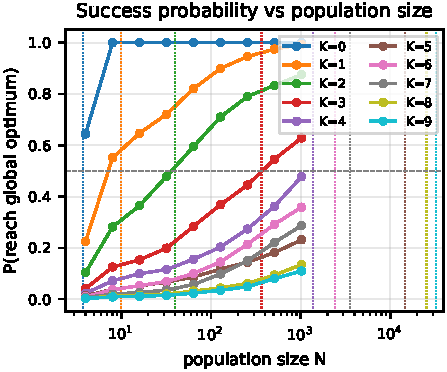
\includegraphics[width=\linewidth]{figures/success_vs_n.pdf}
\caption{Success probability vs. population size, one curve per $K$;
dotted vertical lines mark the fitted $N_c$.}
\label{fig:success}
\end{figure}

\begin{figure}[t]
\centering
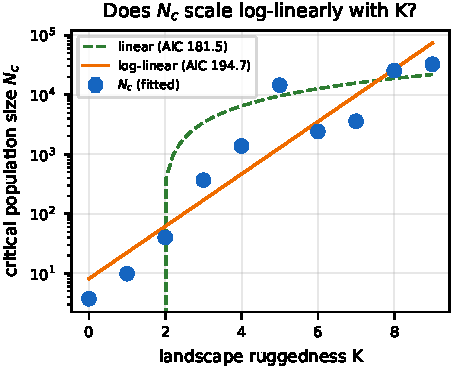
\includegraphics[width=\linewidth]{figures/nc_vs_k.pdf}
\caption{$N_c(K)$ with linear and log-linear fits overlaid (log scale).}
\label{fig:nc}
\end{figure}

\subsection{The mechanism test: falsified, and more cleanly at scale}
Table~\ref{tab:kimura} is the project's central result, now with 10 points
instead of 4. The selection coefficient $s(K)$ increases
\emph{monotonically} across every one of the 10 points ($s(K) \approx
e^{\SFitIntercept + \SSlope K}$), not decreasing as the hypothesis
predicted; consequently $N_c^{\text{Kimura}}(K)$ falls monotonically
(\NcKimuraKZero\ $\to$ \NcKimuraKNine) while the directly-measured $N_c(K)$
rises by three to four orders of magnitude over the same range
(Figure~\ref{fig:kimura}). This is not a small-sample artefact of the
local pilot: the monotonic increase in $s(K)$ is, if anything, cleaner at
this resolution than in the 4-point pilot.

\begin{table}[h]
\centering
\caption{Measured $s(K)$ and $N_c^{\text{Kimura}}(K) = 1/s(K)$.}
\label{tab:kimura}
\small
\begin{tabular}{cccc}
\toprule
$K$ & $s(K)$ & $K$ & $s(K)$ \\
\midrule
0 & \SKZero & 5 & \SKFive \\
1 & \SKOne & 6 & \SKSix \\
2 & \SKTwo & 7 & \SKSeven \\
3 & \SKThree & 8 & \SKEight \\
4 & \SKFour & 9 & \SKNine \\
\bottomrule
\end{tabular}
\end{table}

\begin{figure}[t]
\centering
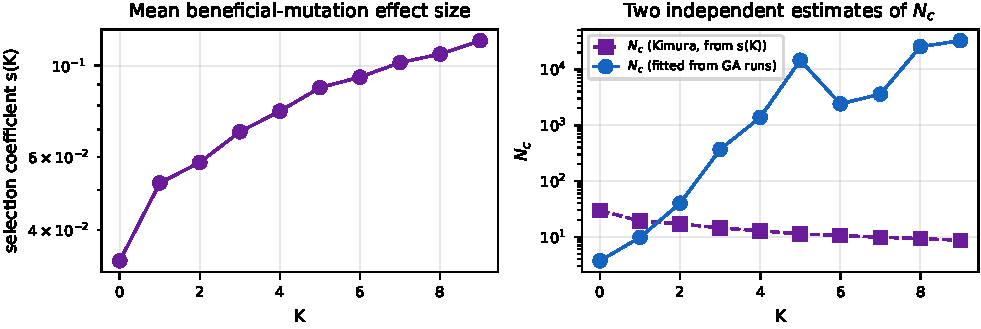
\includegraphics[width=\linewidth]{figures/kimura_check.pdf}
\caption{Left: measured selection coefficient $s(K)$, monotonically
increasing. Right: the two independent $N_c(K)$ estimates, moving in
opposite directions.}
\label{fig:kimura}
\end{figure}

\subsection{Effective population size}
$N_e$, estimated from allele-frequency trajectories at a fixed census
size $N=500$ with no elitism, itself increases with $K$ (roughly 100 at
$K=0$ to 180 at $K=9$) -- the same order of magnitude as $N$ throughout,
confirming the GA remains a reasonable Wright-Fisher-like object to
compare against Kimura's formula at every $K$ tested, not just at $K=0$.
